\section{Image Classification}\label{sec:image-classification}

Image classification is a core task in Computer Vision, based on the problem that a computer ``sees'' an image just like a grid of numbers (\textit{semantic gap}).\\
Furthermore, there are many challenges to face in image classification, not dissimilar to those we discussed for object identification in section \ref{sec:histograms}:
\begin{myitem}
    \item viewpoint variation,
    \item background clutter,
    \item illumination
    \item deformation
    \item occlusion
    \item intraclass variation
\end{myitem}


\subsection{Data driven approaches (machine learning)}\label{sec:ic-ml}

There is no obvious way to hard code an algorithm for recognizing images, even if attempts based on edge detection and corners have been made.\\
Thus, the preferred approach is based on Machine learning:
\begin{myenum}
    \item Collect a dataset of images and labels,
    \item Use Machine Learning to train a classifier,
    \item Evaluate the classifier on new images.
\end{myenum}


\subsection{K Nearest Neighbors classifier}\label{sec:ic-knn}

A first classifier we can consider is \textbf{Nearest Neighbor}. The approach is the following:
\begin{myenum}
    \item Memorize all data and labels;
    \item For each test image:
    \begin{enumerate}
        \item find closest (most similar) train image;
        \item predict label of the nearest image.
    \end{enumerate}
\end{myenum}

With a basic implementation, the training requires $O(1)$ steps, while the prediction $O(N)$, but we want classifiers that are fast at prediction. By the way, many methods exist for fast/approximate nearest neighbor.

To compare images, the \textbf{L1/Manhattan distance metric} is used:
\begin{equation}\label{eq:l1-distance}
    d_1(I_1, I_2) = \sum_p \abs{I_1^p - I_2^p}
\end{equation}
that is, the sum of the pixel-wise absolute value differences between two images.

The idea of \textbf{KNN} is to take the majority vote from $K$ closest points, instead of copying the label of the nearest one (see figure \ref{fig:knn} for an example).

\begin{figure}[!h]
    \centering
    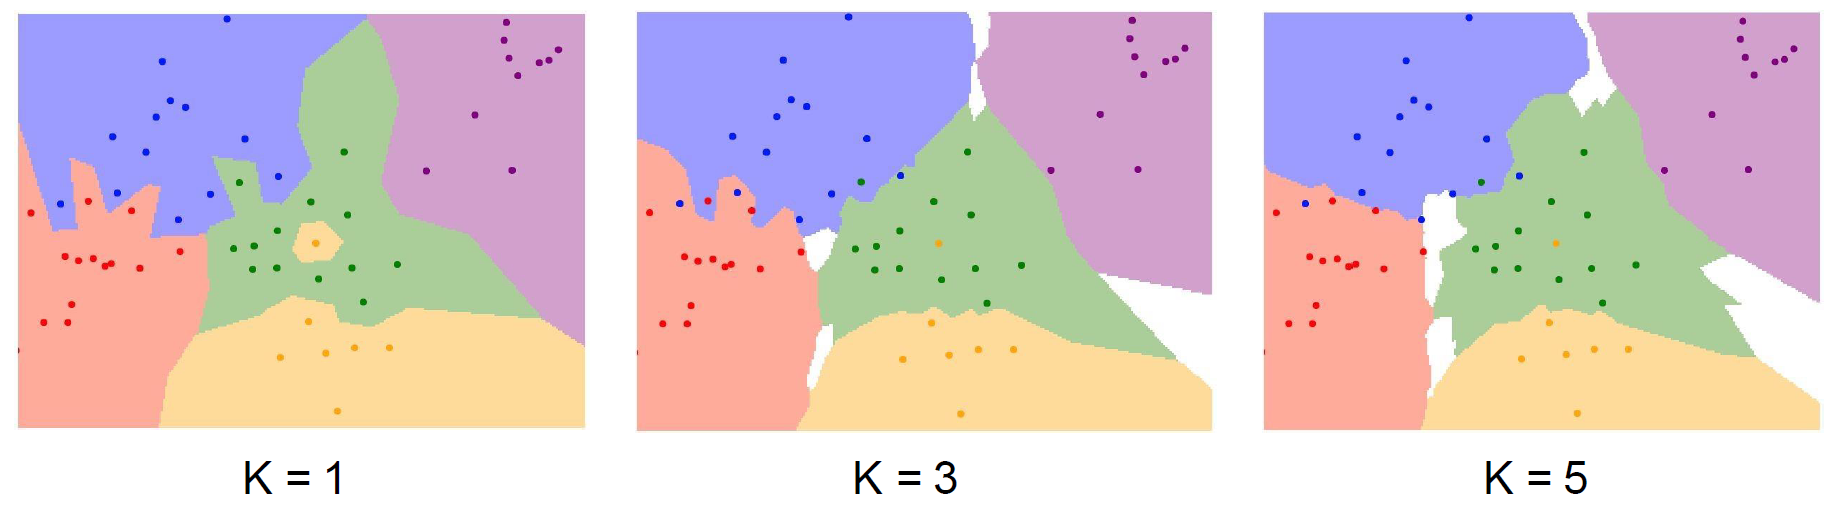
\includegraphics[width=.9\textwidth]{knn}
    \caption[KNN example]{KNN example}
    \label{fig:knn}
\end{figure}

The distance metrics used in KNN are Manhattan like in Nearest Neighbor (see equation \ref{eq:l1-distance}) or \textbf{L2/Euclidean distance}:
\begin{equation}\label{eq:l2-distance}
    d_2(I_1, I_2) = \sqrt{\sum_p \left(I_1^p - I_2^p\right)^2}
\end{equation}

The \textbf{hyperparameters} of a classifier are choices about the algorithm that we set rather than learn, such as the value of $K$ or the distance to use. Since they are problem-dependent, we must try and see what works best.\\
A possibility to find the best hyperparameters is to split the data into \textit{train}, \textit{validation} and \textit{test}, so that we can use the validation set to fine tune the classifier trained on the training set, and then test it on the images of the test set, that it has never seen before.\\
Another possibility is \textbf{k-fold cross validation}: part of the dataset is used as test set, the remaining is divided into $k$ folds, each of which is used as validation set in turn, then the results are averaged (note that this $k$ has nothing to do with the hyperparameter $K$ of KNN). This approach is particularly useful for small dataset.

That said, in practice KNN is never used on images: it is too slow at test time, distance metrics on pixels are not informative, curse of dimensionality (details on this issue \href{https://en.wikipedia.org/wiki/Curse_of_dimensionality}{on Wikipedia}).


\subsection{Linear classification (parametric approach)}\label{sec:ic-linear-classification}

First of all, let's say that Linear classifiers are the building blocks of the Neural Networks.

Given an image represented as a 1D vector $x$ (a flattened matrix of $n$ elements) and $m$ classes, a linear classifier is a function
\begin{equation}\label{eq:linear-classifier}
    f(x,W) = Wx + b
\end{equation}
where $W$ is a matrix of parameters (or \textit{weights}) with $m$ rows and $n$ columns, and $b$ is called \textit{bias}.\\
We can give different interpretation of the linear classifier:
\begin{myitem}
    \item Algebraic viewpoint: we compute a score for each class, based on matrix multiplication;
    \item Geometric viewpoint: we compute hyperplanes cutting up a space of images, to split it according to classes;
    \item Visual viewpoint: we apply to $x$ a template for each class (a row of $W$ can be seen as a template image with the same size of $x$).
\end{myitem}


\subsection{Loss functions and regularization}\label{sec:ic-loss}

At this point, we need a \textit{loss function} that quantifies our unhappiness with the scores across the training data, that is, that tells how good our current classifier is.

Given a dataset of examples
$\left\{\left(x_i, y_i\right)\right\}=N_{i=1}$, where $x_i$ are images and $y_i$ are integer labels, the \textbf{loss over the dataset} is the average of the losses over the examples:
\begin{equation}\label{eq:loss}
    L = \frac1N \sum_i L_i \left( f \left(x_i, W\right), y_i \right)
\end{equation}

Given an example $\left(x_i, y_i\right)$, and a scores vector $s = f \left(x_i, W\right)$, the \textbf{multiclass SVM loss} (or \textit{Hinge loss}) is:
\begin{flalign}\label{eq:svm-loss}
    L_i &= \sum_{j \neq y_i}
    \begin{cases}
        0 &\text{if } s_{y_i} \geq s_j + 1\\
        s_j - s_{y_i} + 1 &\text{otherwise}
    \end{cases}\\
    &= \sum_{j \neq y_i} \max(0, s_j - s_{y_i} + 1) \notag
\end{flalign}
that is, it gives a penalty to each score that is bigger than the score of the correct label + 1.

At this point it is worth noting that this loss isn't unique for a certain $W$, so we need a way to choose the ``best'' $W$ among those with the same loss, thus we introduce \textbf{regularization}:\label{ic-regularization}
\begin{equation}
    L(W) = \underbrace{\frac1N \sum_{i=1}^N L_i \left( f \left(x_i, W\right), y_i \right)}_{\text{data loss}} + \underbrace{\lambda R(W)}_{\text{regularization}}
\end{equation}
where $\lambda$ is a hyperparameter that determines the regularization's strength.\\
The data loss forces the model predictions to match training data, while the regularization prevents the model from doing too well on training data (i.e., avoids overfitting), expresses preferences over weights, makes the model simple so it works on test data, improves optimization by adding curvature.

Examples of regularization are:
\begin{myitem}
    \item L2 regularization
        \begin{equation}\label{eq:l2-regularization}
            R(W) = \sum_k \sum_l W^2_{k,l};
        \end{equation}
    \item L1 regularization:
        \begin{equation}\label{eq:l1-regularization}
            R(W) = \sum_k \sum_l \abs{W_{k,l}};
        \end{equation}
    \item Elastic net (L1 + L2):
        \begin{equation}\label{eq:elastic-net}
            R(W) = \sum_k \sum_l \left( \beta W^2_{k,l} + \abs{W_{k,l}} \right);
        \end{equation}
    \item Dropout;
    \item Batch normalization;
    \item Stochastic depth;
    \item Fractional pooling.
\end{myitem}


\subsection{Softmax classifier (Multinomial Logistic regression)}\label{sec:ic-softmax}

The aim is to interpret raw classifier scores as probabilities.

Given a scores vector $s$, the Softmax function is
\begin{equation}\label{eq:softmax}
    P(y | x_i) = P(Y=k | X = x_i) = \frac{e^{s_k}}{\sum_j e^{s_j}},
\end{equation}
that is, we start with un-normalized log-probabilities (\textit{logits}), we compute the $exp$ to obtain non negative values, and finally we normalize, so that the sum of the values is 1.

In this case, weights are updated with \textbf{maximum likelihood estimation}: choose weights to maximize the likelihood of the observed data. This is done by comparing the computed probabilities with a one-hot vector that gives probability 1 to the true label and 0 to the others. For the comparison three methods can be used:
\begin{myenum}
    \item Entropy:
        \begin{equation}\label{eq:entropy}
            H(P^t) = - \sum_y P^t(y) \log P^t(y)
        \end{equation}
    \item Kullback–Leibler divergence:
        \begin{equation}\label{eq:kl-divergence}
            D_{KL} \left( P^t || Q \right) = \sum_y P^t(y) \log \frac{P^t(y)}{Q(y)}
        \end{equation}
    \item Cross Entropy (the sum of 1 and 2):
        \begin{flalign}\label{eq:cross-entropy}
            H(P^t, Q) &= H(P^t) + D_{KL}(P^t || Q) \\
            &= \sum_y P^t(y) \left( \log \frac{P^t(y)}{Q(y)} - \log P^t(y) \right) \notag\\
            &= - \sum_y P^t(y) \log Q(y) \notag
        \end{flalign}
\end{myenum}
Since the target distribution is 
\begin{equation*}
    P^t(y) =
    \begin{cases}
        1 &y=y_i\\
        0 &y \neq y_i
    \end{cases}
\end{equation*}
and the output of the network is $Q(y | x_i)$ (as given by softmax function \ref{eq:softmax}), the \textit{Cross Entropy Loss} for an image $x_i$, used to maximize the probability of the correct class, is:
\begin{flalign}\label{eq:cross-entropy-loss}
    L_i = L(x_i) &= - \sum_y P^t(y) \cdot \log Q(y | x_i)\\
    &= -1 \cdot \log Q(y | x_i) \notag\\
    &= - \log P(Y=y_i | X=x_i) \notag\\
    &= - \log \frac{e^{s_{y_i}}}{\sum_j e^{s_j}} \notag
\end{flalign}

\obs $L_i \in [0, \infty)\ \forall\ i$.
\obs Since at initialization all $s$ are approximately equal, the loss is $\log(C)$.
\obs Softmax loss reflects more slight changes in the input, thus it is more useful to choose among different values of $W$.


\subsection{Optimization via gradient descent}\label{sec:ic-gradient-descent}

The most common strategy used to optimize weights is \textit{gradient descent}, often represented as a walk from the top of a mountain towards the valley, following the slope (see figure \ref{fig:gradient1}).

As we already mentioned in section \ref{sec:bif-edge}, in one dimension the derivative of a function $f(W)$ is
\begin{equation}\label{eq:derivative}
    \frac{f(W)}{dW} = \lim_{h \to 0} \frac{f(W + h) - f(W)}{h},
\end{equation}
while in multiple dimensions the gradient is the vector of partial derivatives along each dimension.\\
The slope in any direction is the dot product of the direction with the gradient, thus the direction of the steepest descent is the negative gradient (see figure \ref{fig:gradient2}).

\begin{minipage}{.5\linewidth}
    \begin{figure}[H]
        \centering
        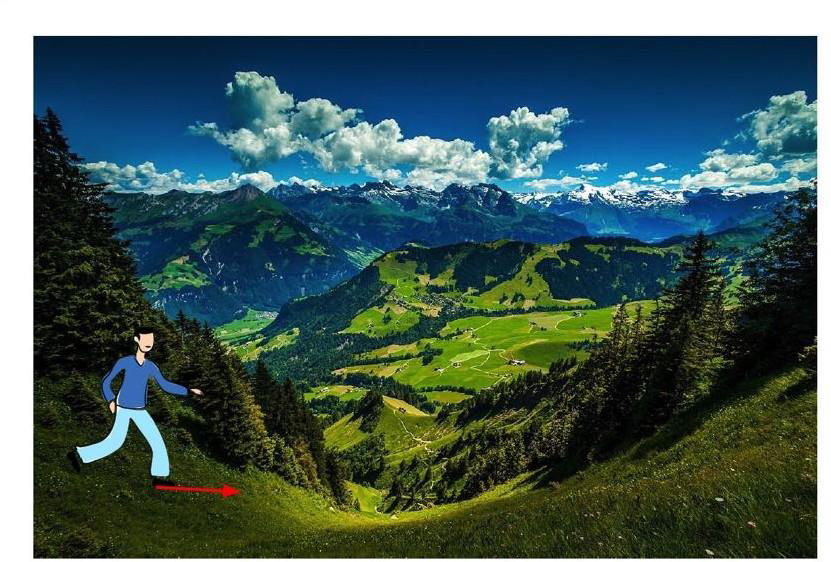
\includegraphics[width=.9\linewidth]{gradient1}
        \caption[Follow the slope]{Follow the slope}
        \label{fig:gradient1}
    \end{figure}
\end{minipage}
\begin{minipage}{.5\linewidth}
    \begin{figure}[H]
        \centering
        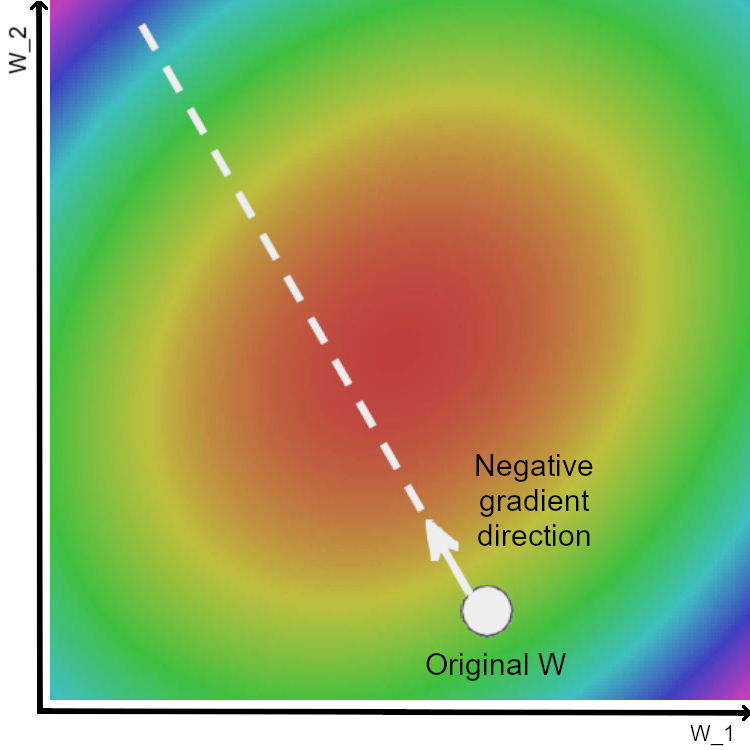
\includegraphics[width=.9\linewidth]{gradient2}
        \caption[Gradient descent]{Gradient descent}
        \label{fig:gradient2}
    \end{figure}
\end{minipage}

To compute the \textbf{numeric gradient} of the loss $\nabla_W L$ requires to loop over all the dimensions of $W$ and apply the formula \ref{eq:derivative} using a fixed small $h$, so it is too slow in practice, and approximate.\\
Since the loss is in fact just a function of $W$, we can use calculus to compute the \textbf{analytic gradient}.\\
In practice, analytic gradient is used for its speed, but its implementation is checked with numerical gradient, since it is more error-prone, although more accurate (\textit{gradient check}).

Let's define the loss as in equation \ref{eq:loss}: $L(W) = \frac1N \sum_i^n L_i(W)$, the computation of the full sum is too expensive when $N$ is large, thus it can be approximated in different ways:\label{bif-sgd}
\begin{myitem}
    \item \textbf{Stochastic Gradient Descent}: randomly choose one training sample $x_i$ and update weights based on loss $L_i(W)$;
    \item \textbf{Mini batch training}: process a subset of training samples $M \subset \{1, \ldots, n\}$ and update weights based on $L_M(W) = \frac{1}{\abs{M}} \sum_{i \in M} L_i(W)$;
    \item \textbf{Batch training} (no approximation): process all training samples update weights based on $L(W)$ (as defined above).
\end{myitem}


\subsection{Image Features}\label{sec:ic-image-features}

To compute class scores for a set of images, it is necessary to adopt an opportune representation of those images. Feature transform can allow to separate points with a linear classifier, even if it wouldn't be possible with the original representation.

Examples of image features are:
\begin{myitem}
    \item \textit{Color histogram} (see section \ref{sec:histograms});
    \item \textit{Histogram of oriented gradients} (divide the image in small regions and quantize edge direction into 9 bins for each region);
    \item \textit{Bag of words}: extract random patches from the images and cluster them to build the \textit{codebook} of visual words, then encode the images based on the occurrences of those patches in them.
\end{myitem}

With Convolutional Neural Networks, the feature extraction phase can be performed within the network itself.


\subsection{Neural Networks and Backpropagation}\label{sec:ic-backpropagation}

As we introduced in section \ref{sec:ic-gradient-descent} there are many problems with manual computation of $\nabla_W L$:
\begin{myitem}
    \item It requires lots of matrix calculus;
    \item If we change loss we have to re-derive from scratch;
    \item Not feasible for very complex models.
\end{myitem}
Thus we use computational graphs and backpropagation. A \textbf{computational graph} is a graph whose edges connect input with functions and functions to outputs. By walking forward on the graph we can compute the loss, and going back we can use \textbf{backpropagation} to compute the gradients. This approach is based on the recursive application of the \textit{Chain rule}, which allows to compute the gradient of a node based on the next two:
\begin{equation}\label{eq:chain-rule}
    \underbrace{\frac{\partial f}{\partial x}}_{\substack{\text{downstream} \\ \text{gradient}}} =
    \underbrace{\frac{\partial f}{\partial q}}_{\substack{\text{upstream} \\ \text{gradient}}} \cdot
    \underbrace{\frac{\partial q}{\partial x}}_{\substack{\text{local} \\ \text{gradient}}}
\end{equation}
where $q$ is the value of the current node, $x$ is the value of the previous node (the one immediately on the left, with the input of the current node), $f$ is the value of the next node (the one immediately on the right, with the output of the current node).

\obs If a node takes more than one input, the gradient propagates on both branches using the Chain rule.

\obs Computational graph representation may not be unique, thus it is important to choose one where local gradients at each node can be easily
expressed.

Patterns in gradient flow (see figure \ref{fig:gradient-pattern}):
\begin{myitem}
    \item Add gate: gradient distributor,
    \item Multiplication gate: swap multiplier,
    \item Copy gate: gradient adder,
    \item Max gate: gradient router.
\end{myitem}

\begin{figure}[!h]
    \centering
    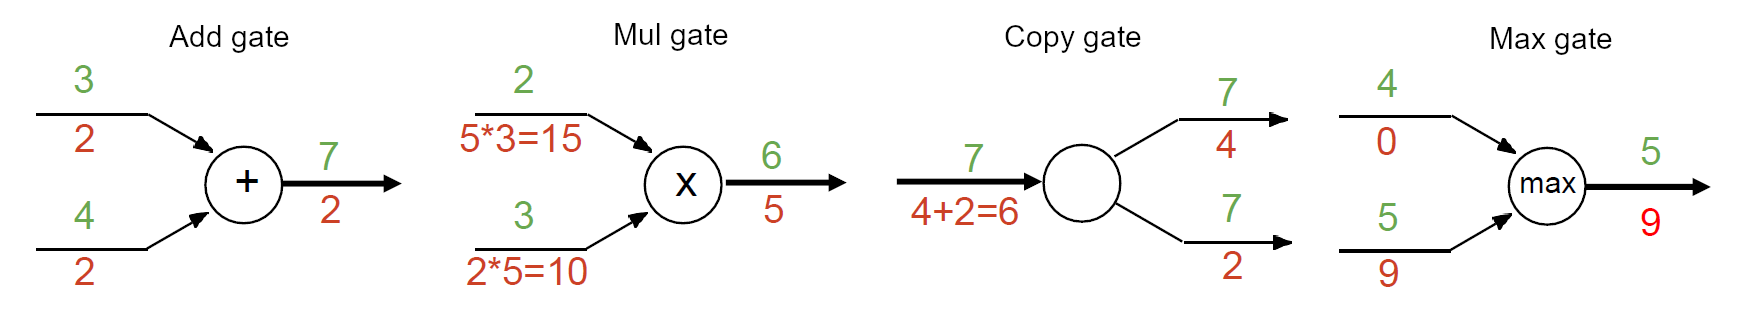
\includegraphics[width=\textwidth]{gradient-pattern}
    \caption[Gradient flow patterns]{Gradient flow patterns}
    \label{fig:gradient-pattern}
\end{figure}

Vector derivatives:
\begin{myitem}
    \item Scalar to scalar: regular derivative
    $\frac{\partial y}{\partial x} \in \mathbb{R}$;
    \item Vector to scalar: derivative is gradient
    $\frac{\partial y}{\partial x} \in \mathbb{R}^N, \ \left(\frac{\partial y}{\partial x}\right)_n = \frac{\partial y}{\partial x_n}$;
    \item Vector to vector: derivative is the \textit{Jacobian matrix}
    $\frac{\partial y}{\partial x} \in \mathbb{R}^{N \times M}, \ \left(\frac{\partial y}{\partial x}\right)_{n,m} = \frac{\partial y_m}{\partial x_n}$.
\end{myitem}

\begin{obs}
    Observations about vector-vector derivatives:
    \begin{myitem}
        \item $\frac{\partial L}{\partial x}$ always has the same shape as $x$.
        \item Since Jacobian is sparse, in fact off-diagonal entries are always zero, it isn't formed explicitly, but only multiplied implicitly.
        \item With an explicit representation Jacobians could take hundreds of GBs of memory.
        \item Let's recall that $y = Wx$, where $x$ is a matrix of size $N \times D$, $W$ is a matrix of size $D \times M$ and $y$ is a matriz of size $N \times M$; then, an element $x_{n,d} \in x$ affects the whole row $y_n$ of $y$, and $x_{n,d}$ affects $y_{n,m}$ by a factor $w_{d,m}$.
        \item Similarly to the previous point, for gradients we have:\\
        \begin{minipage}{.45\linewidth}
            \begin{equation}
                \underbrace{\frac{\partial L}{\partial x}}_{N \times D} = 
                \underbrace{\left(\frac{\partial L}{\partial y}\right)}_{N \times M} \cdot 
                \underbrace{W^T}_{M \times D}
            \end{equation}
        \end{minipage}
        \begin{minipage}{.45\linewidth}
            \begin{equation}
                \underbrace{\frac{\partial L}{\partial W}}_{D \times M} =
                \underbrace{x^T}_{D \times N} \cdot
                \underbrace{\left(\frac{\partial L}{\partial y}\right)}_{N \times M}
            \end{equation}
        \end{minipage}
    \end{myitem}
\end{obs}

